The TUe \acrfull{ed} is a \acrfull{ros} based 3D geometric, object-based world representation system for robots. In itself ED is database system that structures multi-modal sensor information and represents this in an object-based world representation that can be utilized for robot localisation, navigation, manipulation and interaction functions. See Figure \ref{fig:ed} for a schematic overview of ED. %\footnote{\acrshort{ed} is an evolution of \acrfull{wire}, that was created in the FP7 RoboEarth Project. Secondly, ED is utilized within the RoboCup @home competition (also read the \href{https://github.com/tue-robotics/team_description_paper/blob/master/Tech_United_At_Home_TDP_2015.pdf}{TU/e 2015 TDP} for RoboCup). More information, software, installation manual and tutorial can be found on \url{https://github.com/tue-robotics/ed}}
%An elaborate explanation, including tutorials are available at our GitHub website \footnote{\url{http://github.com/tue-robotics}}.
ED is used on our robots AMIGO and SERGIO in the open @Home league and will be used on the Toyota HSR in the DSPL. In previous years, developments have been focussed towards making ED platform independent. As a results ED had been used on the PR2 system, Turtlebot and Dr. Robot systems (X80).
\begin{figure}[h]
    %\vspace{-0.3cm}
	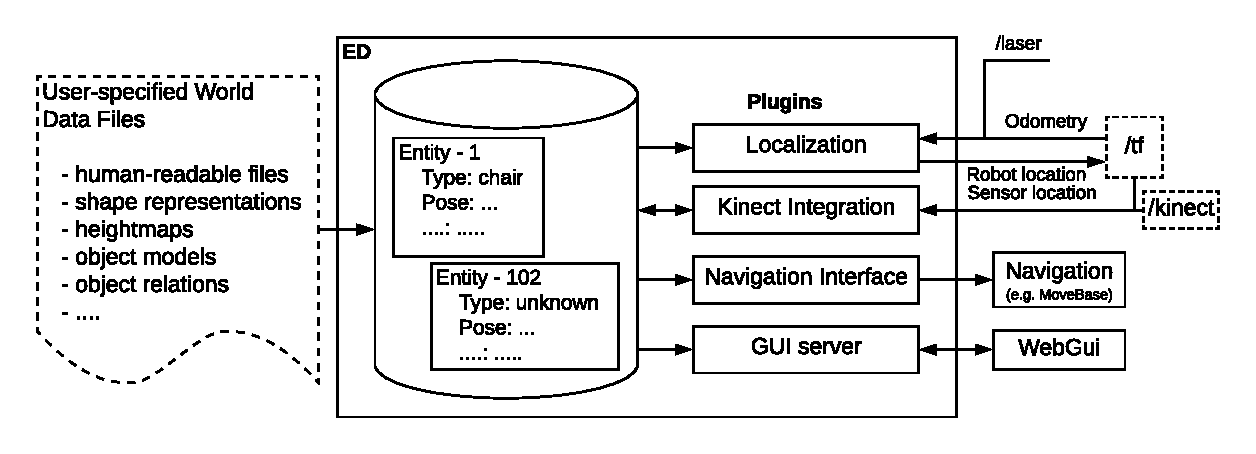
\includegraphics[width = 0.9\linewidth]{Figures/ed_overview}
    %\vspace{-1em}
	\caption{schematic overview of TUe Environment Descriptor.}
	\label{fig:ed}
    %\vspace{-0.5cm}
\end{figure}
ED is one re-usable environment description that can be used for a multitude of needed functionalities. Instead of having different environment representations for localization \acrfull{amcl}, navigation (MoveBase), manipulation (MoveIt!), interaction, etc.. An improvement in this single, central world model will reflect in the performances of the separate robot capabilities. It omits updating and synchronization of multiple world models. At the moment different ED modules exist that enable robots to localize themselves, update positions of known objects based on recent sensor data, segment and store newly encountered objects and visualize all this through a web-based \acrshort{gui}, illustrated in Figure \ref{fig:gui_actions}.
\begin{figure}[h]
\centering
    %\vspace{-0.3cm}
	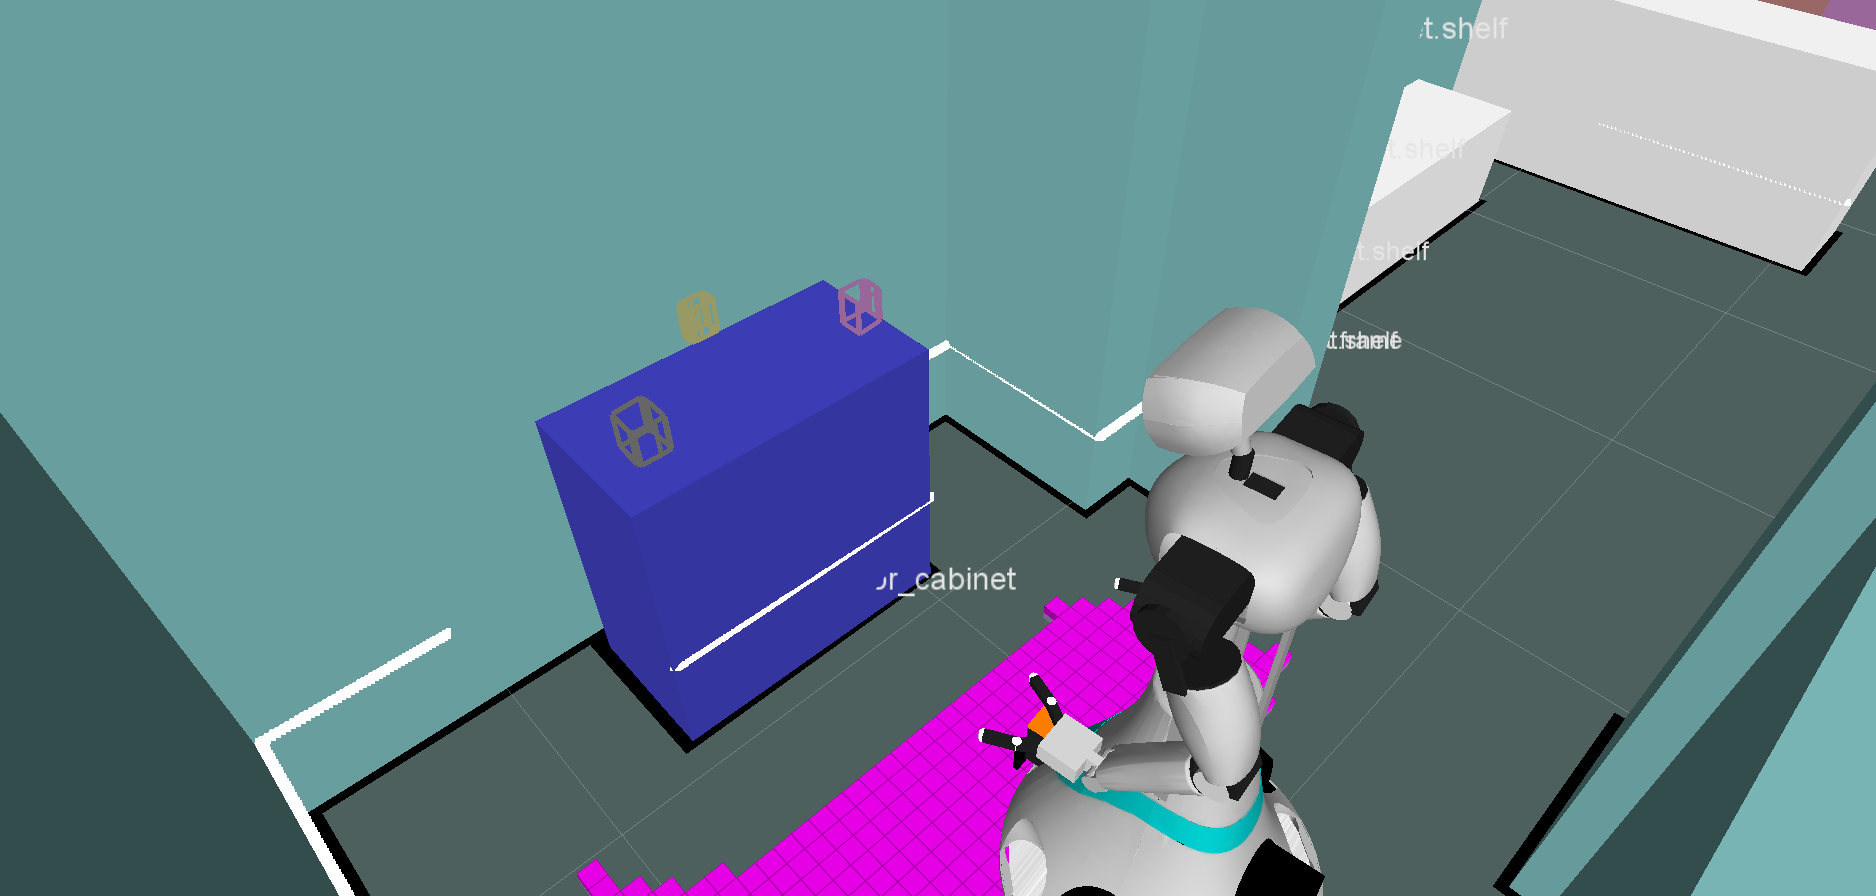
\includegraphics[width = 0.8\linewidth]{Figures/ed_segmentation}
    %\vspace{-0.5em}
	\caption{A view of the world model created with ED. The figure show the occupation grid as well as (unknown) objects recognized on top of the cabinet.}
	\label{fig:ed_segmentation}
    %\vspace{-0.5cm}
\end{figure}

